\chapter{Theoretische Grundlagen}

Um die Funktionsweise von Augmented Reality (AR) und verwandten Technologien zu verstehen, ist ein grundlegendes Wissen über die zugrunde liegenden Konzepte und Techniken erforderlich. In diesem Kapitel werden die theoretischen Grundlagen der Computer Vision und Computergrafik erläutert, die für die Entwicklung von AR-Anwendungen relevant sind. Dabei wird vor der Fokus vor allem auf die Konzepte gelegt, die eine Relevanz für mobile AR-Anwendungen haben. Dazu gehören die Rekonstruktion von 3D-Szenen, die Kamerakalibrierung, die Sensorik, das Tracking und Rendering von virtuellen Objekten.

\section{Drei-dimensionale Computergrafik}

Um Augmented Reality und verwandte Technologien zu verstehen, ist ein grundlegendes Verständnis der mathematischen und geometrischen Prinzipien erforderlich, die der Darstellung und Manipulation dreidimensionaler Objekte zugrunde liegen. Diese Prinzipien bilden die Basis für die Erzeugung und Interaktion mit virtuellen Szenen und Objekten. 

In der Computergrafik werden drei-dimensionale Objekte, auch als Modelle bezeichnet, durch geometrische und relationale Informationen beschrieben. Diese Objekte bestehen in der Regel aus Polygonen, die durch ihre Eckpunkte (Vertices) definiert sind. Ein Polygon ist eine geschlossene Fläche, die durch das Verbinden der Vertices mit geraden Linien entsteht. Ein 3D-Modell wird in einem kartesischen Koordinatensystem beschrieben, wobei die Positionen der Vertices durch ihre \(x\)-, \(y\)- und \(z\)-Koordinaten angegeben werden.

Das einfachste Polygon ist ein Dreieck, das nur drei Eckpunkte benötigt. Dreiecke sind planar und konvex, was sie ideal für Berechnungen in der Computergrafik macht, wie beispielsweise bei der Beleuchtung oder Kollisionserkennung. Obwohl komplexere Polygone existieren, werden diese oft in Dreiecke zerlegt, da sie von Grafikpipelines effizienter verarbeitet werden können. Solche Modelle bestehen dann aus Dreiecksnetzen (Meshes), die als Arrays von Vertices und Indizes gespeichert werden.

Virtuelle 3D-Szenen und Objekte werden in einem kartesischen Koordinatensystem beschrieben. Dieses Koordinatensystem wird üblicherweise als Weltkoordinatensystem bezeichnet, in dem die \(x\)-, \(y\)- und \(z\)-Achsen die drei Dimensionen repräsentieren. In einem rechtshändigen Koordinatensystem zeigt die \(x\)-Achse nach rechts, die \(y\)-Achse nach oben und die \(z\)-Achse nach vorne. Die Position eines Objekts im Raum wird oft mithilfe einer Transformationsmatrix beschrieben.

\section{Matrixalgebra}

Das Anwenden von mathematischen Operationen auf Matrizen ist ein grundlegendes Konzept für viele Algorithmen in der Computer Vision. Diese Arbeit setzt voraus, dass der Leser mit den Grundladen der Matrixalgebra vertraut ist. Im Folgenden werden dennoch die wichtigsten Operationen und Konzepte anhand der Transformationen in der Computergrafik erläutert.

Unter der Transformation eines Objektes in einer 3D-Szene versteht man das Verschieben, Drehen oder Skalieren dieses Objektes. Diese Vorgänge können durch Transformationsmatrizen beschrieben werden, die einheitlich auf alle Vertices eines Objekts angewendet werden. Solche Matrizen haben typischerweise die Größe \(4 \times 4\) und kombinieren Translation, Rotation und Skalierung. Dies hat den Vorteil, dass alle Transformationen in einer einzigen Matrix zusammengefasst werden können, was die Berechnungen effizienter macht.

\subsection{Translation}

Die Translation verschiebt ein Objekt entlang der \(x\)-, \(y\)- oder \(z\)-Achse. Die Transformationsmatrix für eine Translation ist wie folgt definiert:

\begin{equation}
\begin{bmatrix}
x' \\ y' \\ z' \\ 1
\end{bmatrix}
=
\begin{bmatrix}
1 & 0 & 0 & t_x \\
0 & 1 & 0 & t_y \\
0 & 0 & 1 & t_z \\
0 & 0 & 0 & 1
\end{bmatrix}
\begin{bmatrix}
x \\ y \\ z \\ 1
\end{bmatrix}
\end{equation}

Hierbei verschieben die Parameter \(t_x\), \(t_y\) und \(t_z\) das Objekt entlang der jeweiligen Achsen.

\subsection{Rotation}

Die Rotation eines Objekts erfolgt um eine der drei Achsen (\(x\), \(y\) oder \(z\)). Die Rotationsmatrizen sind für jede Achse wie folgt definiert:

\paragraph{Rotation um die \(x\)-Achse:}
\begin{equation}
\begin{bmatrix}
1 & 0 & 0 & 0 \\
0 & \cos(\alpha) & -\sin(\alpha) & 0 \\
0 & \sin(\alpha) & \cos(\alpha) & 0 \\
0 & 0 & 0 & 1
\end{bmatrix}
\end{equation}

\paragraph{Rotation um die \(y\)-Achse:}
\begin{equation}
\begin{bmatrix}
\cos(\alpha) & 0 & \sin(\alpha) & 0 \\
0 & 1 & 0 & 0 \\
-\sin(\alpha) & 0 & \cos(\alpha) & 0 \\
0 & 0 & 0 & 1
\end{bmatrix}
\end{equation}

\paragraph{Rotation um die \(z\)-Achse:}
\begin{equation}
\begin{bmatrix}
\cos(\alpha) & -\sin(\alpha) & 0 & 0 \\
\sin(\alpha) & \cos(\alpha) & 0 & 0 \\
0 & 0 & 1 & 0 \\
0 & 0 & 0 & 1
\end{bmatrix}
\end{equation}

Die Reihenfolge, in der Rotationen um verschiedene Achsen durchgeführt werden, ist entscheidend, da sie die endgültige Orientierung beeinflusst. Diese Reihenfolge wird durch Euler-Winkel beschrieben.

\subsection{Skalierung}

Die Skalierung verändert die Größe eines Objekts proportional entlang der \(x\)-, \(y\)- und \(z\)-Achsen. Die Skalierungsmatrix ist wie folgt definiert:

\begin{equation}
\begin{bmatrix}
x' \\ y' \\ z' \\ 1
\end{bmatrix}
=
\begin{bmatrix}
s_x & 0 & 0 & 0 \\
0 & s_y & 0 & 0 \\
0 & 0 & s_z & 0 \\
0 & 0 & 0 & 1
\end{bmatrix}
\begin{bmatrix}
x \\ y \\ z \\ 1
\end{bmatrix}
\end{equation}

Hierbei sind \(s_x\), \(s_y\) und \(s_z\) die Skalierungsfaktoren entlang der jeweiligen Achsen.

\subsection{Anwendung der Transformationen}

Die lokalen Koordinaten eines Objekts können mithilfe einer Transformationsmatrix in Weltkoordinaten umgerechnet werden:

\begin{equation}
P_{world} = T_{object} \cdot P_{object}
\end{equation}

Hierbei ist \(T_{object}\) die Transformationsmatrix des Objekts, und \(P_{object}\) sind die lokalen Koordinaten. Das Ergebnis \(P_{world}\) beschreibt die Position des Objekts im Weltkoordinatensystem.

\section{Kalibrierung}

In Augmented-Reality-Anwendungen ist eine präzise Überlagerung digitaler Informationen auf die reale Welt essenziell, um ein realistisches und funktionales Benutzererlebnis zu schaffen. Die Kamerakalibrierung spielt hierbei eine entscheidende Rolle, da sie sicherstellt, dass virtuelle Objekte korrekt positioniert, skaliert und perspektivisch angepasst in die physische Umgebung integriert werden.

Die Kalibrierung umfasst die Bestimmung der \textbf{intrinsischen} und \textbf{extrinsischen} Parameter der Kamera:

\begin{itemize}
    \item \textbf{Intrinsische Parameter} beschreiben die optischen Eigenschaften der Kamera, wie Brennweiten, Verzerrungen und die Position des optischen Zentrums.
    \item \textbf{Extrinsische Parameter} legen die Position und Orientierung der Kamera im Raum fest, was für die korrekte Transformation zwischen Welt- und Bildkoordinaten erforderlich ist.
\end{itemize}

\begin{figure}
    \centering
    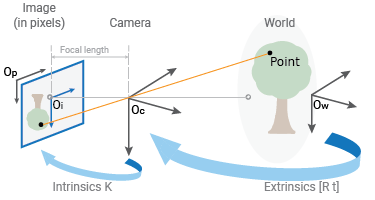
\includegraphics[ width=.5\textwidth ]{calibration-cameramodel-coords}
    \caption{Modell für die Kamerakalibrierung\label{fig:Kalibrierung}}\par
\end{figure}

Mathematisch wird die Transformation durch die Gleichung \( x = PX \) beschrieben, wobei:

\begin{itemize}
    \item \( x \) die Bildkoordinaten in Pixeln sind,
    \item \( P \) die Projektionsmatrix ist und
    \item \( X \) die Weltkoordinaten eines Objekts darstellt.
\end{itemize}

Die Projektionsmatrix \( P \) setzt sich aus der intrinsischen Matrix \( K \) sowie der Rotationsmatrix \( R \) und dem Translationsvektor \( t \) zusammen:
\[
P = K[R|t]
\]

Die intrinsische Matrix \( K \) wird folgendermaßen definiert:
\[
K = 
\begin{bmatrix}
f_x & s & c_x \\
0 & f_y & c_y \\
0 & 0 & 1
\end{bmatrix}
\]
\begin{itemize}
    \item \( f_x \) und \( f_y \): Brennweiten der Kamera in Pixeln, bezogen auf die horizontalen und vertikalen Achsen.
    \item \( c_x \) und \( c_y \): Koordinaten des optischen Zentrums in Pixeln.
    \item \( s \): Skew-Faktor, der berücksichtigt, ob die Kameraachsen orthogonal sind.
\end{itemize}

Die Transformation von Weltkoordinaten in Bildkoordinaten wird schließlich durch die Matrix-Multiplikation berechnet:
\[
\begin{bmatrix}
x \\ y \\ 1
\end{bmatrix}
= 
\begin{bmatrix}
f_x & 0 & c_x \\
0 & f_y & c_y \\
0 & 0 & 1
\end{bmatrix}
\begin{bmatrix}
r_{11} & r_{12} & r_{13} & t_1 \\
r_{21} & r_{22} & r_{23} & t_2 \\
r_{31} & r_{32} & r_{33} & t_3
\end{bmatrix}
\begin{bmatrix}
X \\ Y \\ Z \\ 1
\end{bmatrix}
\]

Zur Kalibrierung werden in der Praxis oft visuelle Marker, wie Schachbrettmuster oder Würfel mit bekannten Geometrien, verwendet. Die Kamera erfasst diese Marker, und mithilfe einer Optimierung, z. B. durch Minimierung eines Fehlermaßes (Loss-Funktion), werden die Kameraparameter berechnet.

Um die Lens-Distortion zu korrigieren, werden oft Polynommodelle, wie das Brown-Conrady-Modell, verwendet. Dieses Modell beschreibt die radiale und tangentialen Verzerrungen der Linse und wird durch die Koeffizienten \( k_1, k_2, k_3 \) und \( p_1, p_2 \) definiert.

Moderne AR-Plattformen wie ARKit oder ARCore integrieren den Kalibrierungsprozess automatisch. ARKit speichert intrinsische Parameter in der Klasse \texttt{AVCameraCalibrationData} und berechnet die extrinsischen Parameter durch die Inertial Measurement Unit (IMU) des Geräts, welche Positions- und Orientierungsdaten liefert.

\section{Sensorik}

Die Erfassung der Umgebung in Augmented-Reality-Anwendungen erfolgt mithilfe verschiedener Sensoren, die Daten über die physische Welt liefern. Je nach Anwendungsfall und Eingabegerät können unterschiedliche Sensoren verwendet werden, um die Position und Bewegung des Geräts zu bestimmen. Zu den wichtigsten Sensoren für mobile AR-Anwendungen gehören:

\begin{itemize}
    \item \textbf{Kamera}: Die Kamera liefert visuelle Informationen über die Umgebung und wird zur Erkennung von Markern, Features oder Objekten verwendet.
    \item \textbf{Gyroskop}: Das Gyroskop misst die Winkelgeschwindigkeit des Geräts und wird zur Erfassung von Drehbewegungen verwendet.
    \item \textbf{Beschleunigungsmesser}: Der Beschleunigungsmesser misst die Beschleunigung des Geräts und wird zur Erfassung von linearen Bewegungen verwendet.
    \item \textbf{Magnetometer}: Das Magnetometer misst das Magnetfeld des Geräts und wird zur Bestimmung der Ausrichtung im Raum verwendet.
    \item \textbf{GPS}: Das GPS (Global Positioning System) bestimmt die geografische Position des Geräts und wird zur Navigation und Lokalisierung verwendet.
\end{itemize}

Sensoren wie Gyroskop, Beschleunigungsmesser und Magnetometer werden oft in einem sogenannten IMU (Inertial Measurement Unit) kombiniert, um die Bewegung des Geräts in sechs Freiheitsgraden (3D-Position und -Orientierung) zu erfassen. 

Bei vielen Tracking-Verfahren werden eine Kombination von Sensoren verwendet, um die Genauigkeit und Zuverlässigkeit der Positionsschätzung zu verbessern. Beispielsweise kann die Kamera für visuelle Tracking-Anwendungen verwendet werden, während das IMU für die Schätzung der Bewegung des Geräts verwendet wird. Durch die Fusion von Daten aus verschiedenen Sensoren können AR-Anwendungen eine präzise und konsistente Darstellung der virtuellen Objekte in der realen Welt erreichen.

\section{Structure from Motion}

Structure from Motion (SfM) ist eine Technik aus der Computer Vision, die verwendet wird, um die 3D-Struktur einer Szene aus einer Reihe von 2D-Bildern zu rekonstruieren. SfM basiert auf der Triangulation von Punkten, die in verschiedenen Bildern sichtbar sind, um die Positionen der Sensoren und der Punkte in der Szene zu bestimmen.

Der Prozess der SfM besteht aus den folgenden Schritten: 

\begin{enumerate}
    \item Feature Detection
    \item Feature Matching
    \item Camera Pose Estimation
    \item 3D Reconstruction
    \item Bundle Adjustment
\end{enumerate}

Diese Schritte werden im Folgenden näher erläutert.

\subsection{Feature Detection und Matching}

Bei der Feature Detection bzw. beim Feature Maching werden Merkmale in verschiedenen Bildern identifiziert und korrespondierende Merkmale gefunden. Dieser Schritt ist entscheidend, um die Bewegung der Kamera (Tracking) und die 3D-Struktur der Szene zu bestimmen. Es gibt verschiedene Algorithmen, die für das Erkennen und Nachverfolgen von Feature-Punkten verwendet werden können, wie z. B. SIFT (Scale-Invariant Feature Transform), SURF (Speeded-Up Robust Features) oder ORB (Oriented FAST and Rotated BRIEF). Diese Algorithmen setzen sich grundsätzlich aus drei Teilen zusammen:

\begin{itemize}
    \item Feature Detector oder Keypoint Detector: Der Feature Detector identifiziert Punkte im Bild, die einzigartige und kontrastreiche Strukturen aufweisen. Diese Punkte werden als Features bezeichnet und dienen als Referenzpunkte für die spätere Berechnung der Kameraposition.
    \item Feature Descriptor: Der Feature Descriptor berechnet eine Beschreibung für jedes Feature, die es ermöglicht, die Features in verschiedenen Bildern zu vergleichen. Diese Beschreibungen sind normalerweise Vektoren, die die Helligkeitsverteilung um den Feature-Punkt herum beschreiben.
    \item Feature Matching Algorithm: Der Feature Matching Algorithmus vergleicht die Feature-Deskriptoren in verschiedenen Bildern, um die korrespondierenden Features zu finden. Diese korrespondierenden Features werden dann verwendet, um die Kameraposition zu schätzen.  
\end{itemize}


Da ORB heutzutage eine große Relevanz aufgrund seiner Effizienz und Robustheit hat, wird dieser Algorithmus im Folgenden näher erläutert:

ORB baut auf den Algorithmen FAST (Features from Accelerated Segment Test) und BRIEF (Binary Robust Independent Elementary Features) auf. Der FAST-Algorithmus wird eingesetzt, um Punkte zu finden, die eine starke Helligkeitsänderung aufweisen. Dabei werden benachbarte Pixel in einem Kreis um den zu prüfenden Pixel verglichen. Wenn die Anzahl von Pixeln in dem Kreis heller oder dunkler ist als der zentrale Pixel größer ist als ein Schwellwert /(T/), wird dieser als Feature-Punkt erkannt. Anschließend wird mithilfe des BRIEF-Algorithmus binäre Deskriptoren berechnet, um die Merkmale zu beschreiben. BRIEF ist ein schneller Algorithmus, der binäre Deskriptoren erzeugt, indem er zufällige Paare von Pixeln auswählt und deren Helligkeitsunterschiede vergleicht. Diese binären Deskriptoren sind effizienter zu berechnen und zu speichern als herkömmliche Deskriptoren. Zuletzt wird FLANN (Fast Library for Approximate Nearest Neighbors) verwendet, um die Merkmale zu gruppieren und zu speichern.

Neben klassischen Algorithmen werden vermehrt auch Deep-Learning-Modelle, wie Convolutional Neural Networks (CNNs), für das Feature Matching eingesetzt. Beispiele dafür sind das XFeat-Model (Accelarated Features), bei dem ein optimiertes Deep Learning neuronales Netzwerk eingesetzt wird, oder OmniGlue, bei dem auf Transformatoren und CNNs gesetzt wird.

\subsection{Camera Pose Estimation}

Die Kamerapositionsschätzung ist ein wichtiger Schritt in der Structure-from-Motion-Pipeline, da sie die Position und Orientierung der Kamera in jedem Bild bestimmt. Dies ist entscheidend, um die 3D-Struktur der Szene zu rekonstruieren und die extrinsischen Parameter der Kamera zu verfolgen. Gehen wir davon aus, dass die intrinsischen Parameter der Kamera bekannt sind und wir mehrere Bilder mit korrespondierenden Punkten zur Verfügung haben, dann kann die Kameraposition mithilfe einer sogenannten Essential Matrix /(E/) geschätzt werden. Diese Matrix beschreibt die Beziehung zwischen den Bildern und ermöglicht es, die Rotation und Translation der Kamera zu berechnen. Die Bedingung, die gelten muss, so dass die Berechnung der extrinsischen Parameter möglich ist, lautet:

\[ x'^T E x = 0 \]

Diese Bedingung bezieht sich auf die Kollinearität der Punkte in den beiden Bildern. Hierbei sind \( x \) und \( x' \) die korrespondierenden Punkte in den beiden Bildern. Anhand dieser Bedingung kann die Essential Matrix mithilfe des Five-Point-Algorithmus (im kalibrierten Fall) geschätzt werden. Der Five-Point-Algorithmus ist eine effiziente Variante, die die Essential Matrix aus mindestens 5 korrespondierenden Punkten schätzt. Die Essential Matrix kann dann mithilfe der Singulärwertzerlegung (SVD) in die Rotations- und Translationsmatrix der Kamera zerlegt werden:

\[E = R [t]_x\]

\subsection{Drei-dimensionale Rekonstruktion}

Bei der drei-dimensionalen Rekonstruktion der Szene werden die zwei-dimensionalen Daten der Kamera in ein dreidimensionales Modell überführt. Dabei werden sowohl die Parameter der Kamera als auch die Translation und Rotation dieser, sowie die korrespondierenden Feature-Punkte aus dem Feature Matching verwendet, um die Positionen der Punkte im Raum zu bestimmen und somit eine 3D-Rekonstruktion der Szene zu erstellen.

Mithilfe der Triangulation können die kartesischen Koordinaten eines Feature-Punktes im Weltkoordinatensystem bestimmt werden. Ein einfaches Verfahren zur Lösung dieses Problems besteht darin, den 3D-Strahlen, die durch die Kamerazentren \( c_j \) in die Richtung \( \hat{v_j} \) verlaufen, zu folgen und den Punkt \( p_0 \) zu finden, der am nächsten an allen Strahlen liegt. Die Richtung \( \hat{v_j} \) wird durch Transformation der 2D-Bildpunkte mit den Kameramatrizen beschrieben. Der Punkt \( p_0 \) weist einen minimalen Abstand zu allen Strahlen auf, so dass dieser z.B. mithilfe der Minimierung der quadratischen Abstände zwischen den Strahlen und dem Punkt berechnet werden kann.

\begin{figure}
    \centering
    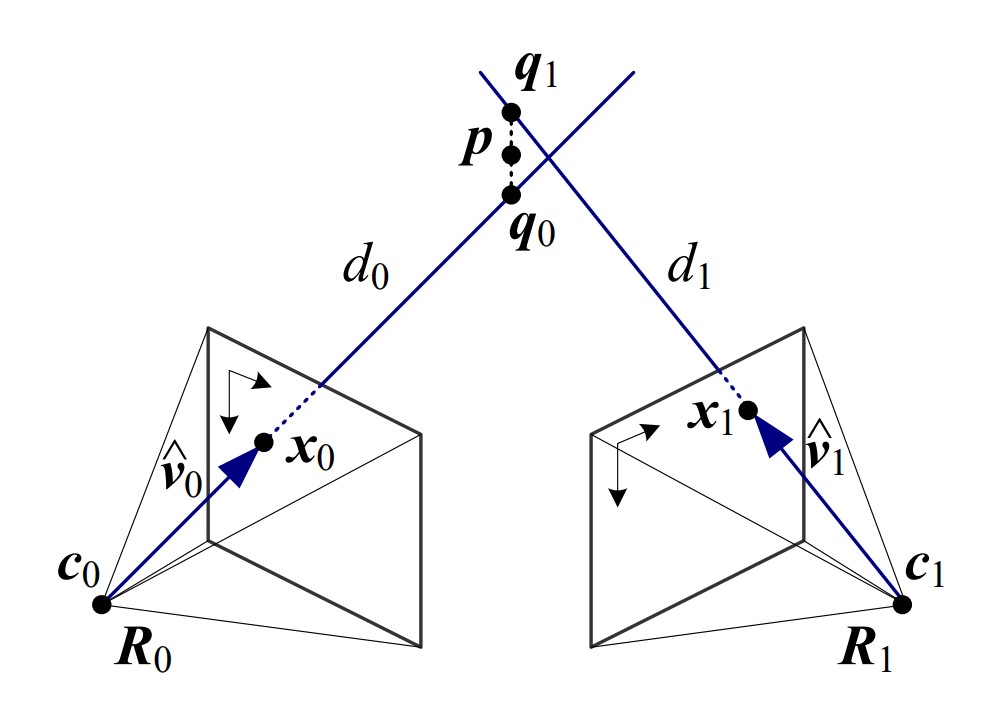
\includegraphics[ width=.5\textwidth ]{Triangulation}
    \caption{Drei-dimensionale Triangulation mit zwei Bildern\label{fig:Triangulation}}\par
\end{figure}

Die Abbildung \ref{fig:Triangulation} stellt die Triangulation eines Punktes im drei-dimensionalen Raum grafisch dar. Mathematisch wird die Triangulation durch die folgende Gleichung beschrieben:

\[
p = \left( \sum_j \left( I - \hat{v_j} \hat{v_j}^T \right) \right)^{-1} \left( \sum_j \left( I - \hat{v_j} \hat{v_j}^T \right) c_j \right)
\]

Das Ergebnis der Triangularisierung der Punkte ist eine sogenannte Punktwolke (Point-Cloud; siehe \ref{fig:PointCloud}), die die 3D-Struktur der Szene repräsentiert. Diese Punktwolke kann dann weiterverarbeitet werden, um ein detailliertes 3D-Modell der Szene zu erstellen. Dazu gehört zum Beispiel die Oberflächenrekonstruktion (engl. Plane Detection), bei der die Punktwolke in Flächen unterteilt wird, um die Oberflächen von Objekten im Raum zu bestimmen. Die Plane-Detection kann mithilfe des RANSAC-Algorithmus (Random Sample Consensus) durchgeführt werden, der Ausreißer in den Daten identifiziert und die Flächen anhand der verbleibenden Punkte schätzt.

\begin{figure}
    \centering
    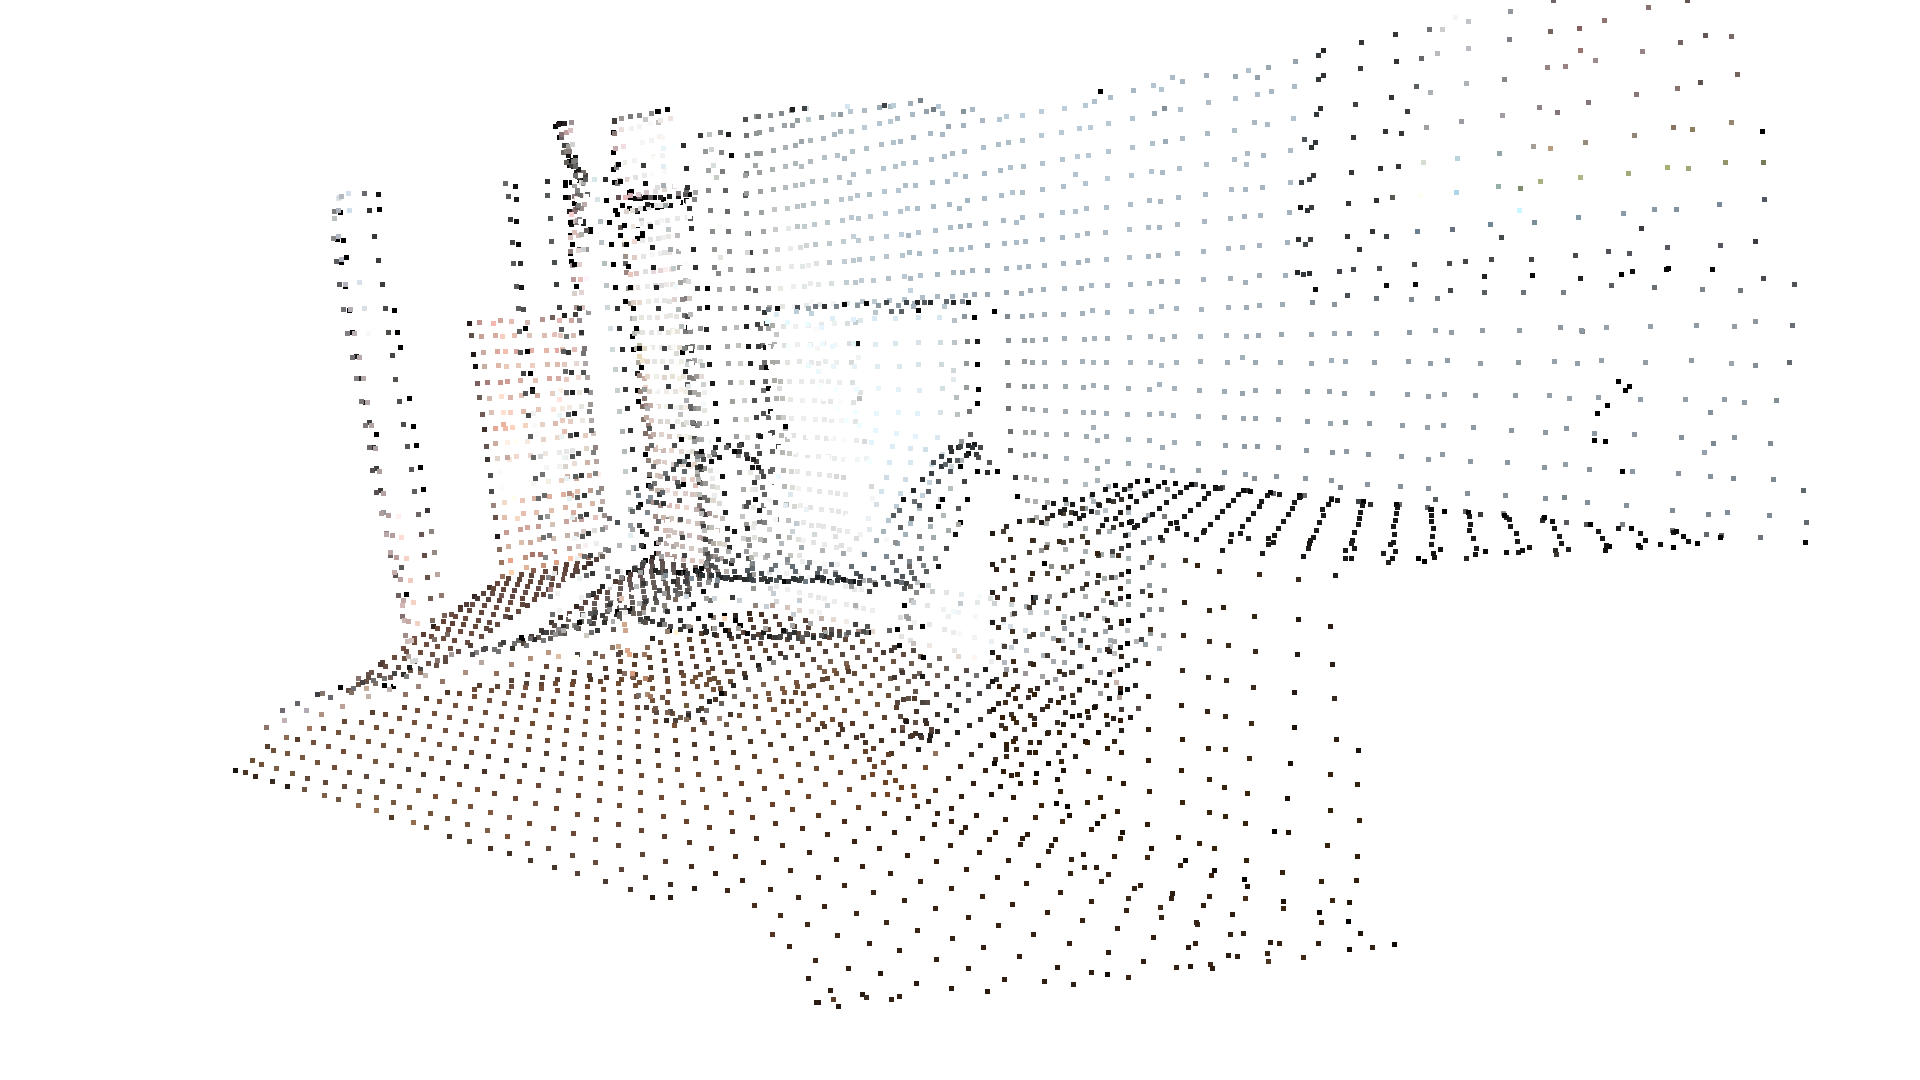
\includegraphics[ width=.5\textwidth ]{PointCloud}
    \caption{Beispiel einer drei-dimensionalen Point-Cloud-Rekonstruktion\label{fig:PointCloud}}\par
\end{figure}

\subsection{Bundle Adjustment}

Der Bundle Adjustment ist ein Optimierungsverfahren, das verwendet wird, um die Kamerapositionen und die 3D-Struktur der Szene zu verfeinern. Dabei werden die Fehler zwischen den projizierten 3D-Punkten und den tatsächlichen 2D-Punkten minimiert, um die bestmögliche Schätzung der Kamerapositionen und der 3D-Struktur zu erhalten. Der Bundle Adjustment ist ein iterativer Prozess, der normalerweise auf der nicht-linearen Optimierung basiert. Es gibt verschiedene Algorithmen zur Bundle Adjustment, wie z. B. die Levenberg-Marquardt-Methode oder die Gauss-Newton-Methode.

\section{Markenbasiertes Tracking}

Beim markenbasierten Tracking werden Feature-Punkte in der echten Welt platziert und anschließend von der Kamera erkannt. In der Abbildung \ref{fig:Marker} ist ein Beispiel für ein markerbasiertes Tracking dargestellt. 

\begin{figure}
    \centering
    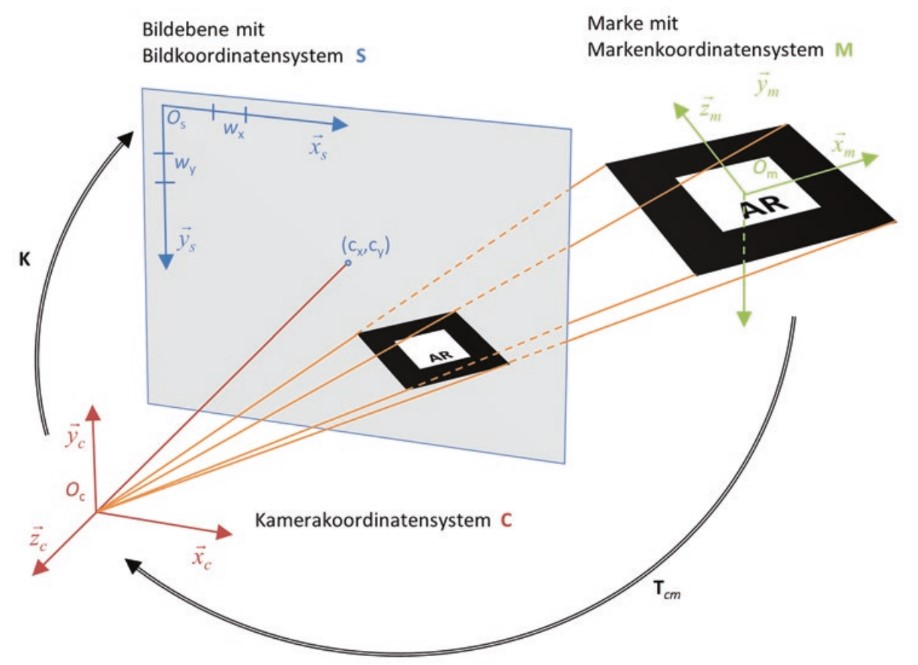
\includegraphics[ width=.5\textwidth ]{Marker}
    \caption{Darstellung eines markenbasiertes Tracking\label{fig:Marker}}\par
\end{figure}

Hier wird mithilfe der intrinsichen und extrinsischen Parameter der Kamera (siehe Kapitel 4.2) die Position und Orientierung des Markers im Raum bestimmt. Dabei nimmt man sich die bekannten Dimensionen des Markers zu Nutze, um eine Transformationsmatrix \(T_cm\) zu berechnen, mithilfe derer man die Koordinaten des Markers im lokalen Koordinatensystem ins Kamerakoordinatensystem transformieren kann. Die Bestimmung der Transformation \(T_cm\) erfolgt funktioniert wie folgt:

Es soll gelten:
\[ v_c = T_cm * v_m \]

Nun gilt für einen Bildpixel \(v_s\) unter Anwendung der intrinsischen Kameraparameter (siehe Kapitel 4.2):
\[ v_s = K * v_c \]

Daraus folgt:
\[ v_s = K * T_cm * v_m \]

Da \(v_s\) und \(v_m\) bekannt sind (die Pixelkoordinaten des Markers und die bekannten Dimensionen des Markers), kann die Transformation \(T_cm\) berechnet werden.

Das markerbasierte Tracking ist besonders robust und präzise, da die Position und Orientierung des Markers bekannt sind. Allerdings ist es auch aufwendiger, da die Marker manuell platziert und kalibriert werden müssen. Es wird häufig in Anwendungen eingesetzt, bei denen die Position des darzustellenden Objekts genau bekannt ist. Auch in der Filmproduktion wird markerbasiertes Tracking oft für Motion-Caputre-Verfahren verwendet.

\section{SLAM}

Simultaneous Localization and Mapping (SLAM) ist eine Technik, die verwendet wird, um die Position und Orientierung eines mobilen Roboters in Echtzeit zu bestimmen, während er eine unbekannte Umgebung erkundet. SLAM basiert auf der Triangulation von Punkten, die in verschiedenen Bildern sichtbar sind, um die Position des Roboters und die 3D-Struktur der Umgebung zu bestimmen.

Der Prozess der SLAM besteht aus den folgenden Schritten:

\begin{enumerate}
    \item Feature Detection
    \item Feature Matching
    \item Camera Pose Estimation
    \item 3D Reconstruction
    \item Loop Closure Detection
    \item Map Optimization
\end{enumerate}

Diese Schritte werden im Folgenden näher erläutert.

\subsection{Loop Closure Detection}

\section{Scene Understanding}

\section{Rendering}

\section{Limitationen}
- anfällig für schlechte Lichtverhältnisse, sich schnell ändernde Umgebungen und sich wiederholenden Strukturen



